\documentclass[a4paper, oneside, onecolumn, 11pt]{article}

\usepackage[spanish]{babel}
\usepackage[utf8]{inputenc}
\usepackage{graphicx}
\usepackage{amsmath, amsthm, amsfonts}
\usepackage{eurosym}
\usepackage{vmargin}
\usepackage[export]{adjustbox}
\usepackage{xcolor}
\usepackage{lineno}
\usepackage[framemethod=tikz]{mdframed}
\usepackage{setspace}
\usepackage{listings} % para poder hacer uso de "listings" propios (p.ej. códigos)
\usepackage{eurosym} % para poder usar el símbolo del euro con \euro {xx}
\usepackage{hyperref}
\usepackage{caption}
\usepackage{siunitx}
\usepackage{authblk}

\usepackage{caption}
\usepackage{subcaption}

\definecolor{cccolor}{rgb}{.67,.7,.67}

\DeclareCaptionType{code}[Code][Code list]

\setmargins{2.5cm}	% margen izquierdo
{1.5cm}			% margen superior
{16.5cm}		% anchura del texto
{23.42cm}		% altura del texto
{10pt}			% altura de los encabezados
{1cm}			% espacio entre el texto y los encabezados
{0pt}			% altura del pie de página
{2cm}			% espacio entre el texto y el pie de página

\begin{document}

\title{\huge{BusVigia 2.0: detección de infracciones en carril bus}}

\author[1,*]{Javier Martínez}
\affil[1]{Universidad Rey Juan Carlos, j.martinezma.2018@alumnos.urjc.es}
\date{\today}

\maketitle

%\onehalfspace
%\doublespacing
\singlespace

\section{Introducción}
\label{sec:intro}

Las ciudades de gran escala se ven continuamente afectadas por problemas de tráfico como atascos o accidentes, lo que provoca que la movilidad sufra fuertes demoras. Una posible solución radica en la correcta gestión del transporte público. Los autobuses urbanos son los más afectados por el tráfico de la ciudad, debido a que comparten la calzada con vehículos privados.

Los carriles exclusivos para autobuses se han diseñado con el objetivo de mejorar la eficiencia del transporte público y el flujo general del tráfico. Sin embargo, estos carriles suelen ser ocupados por vehículos privados y los autobuses se ven obligados a utilizar los carriles comunes. Para evitar este problema se instalan separadores físicos sobre la línea del carril bus que, a pesar de ser una solución satisfactoria, son peligrosos y provocan accidentes.

En \cite{FernandezLopez2013} se presenta un sistema basado en visión artificial capaz de detectar, de forma automática, vehículos que obstaculizan el carril bus. El sistema se instala en los autobuses y consigue un gran efecto disuasorio, debido a que todas las infracciones captadas son sancionadas con una multa. El uso de esta tecnología hace que ya no sean necesarios los separadores físicos, lo que mejora la movilidad general y la seguridad vial de las ciudades.

El algoritmo usado en \cite{FernandezLopez2013} está basado en técnicas clásicas de procesamiento de imágenes. En la última década, la visión artificial ha experimentado un gran auge en cuanto a precisión debido a los nuevos métodos basados en aprendizaje profundo. En este trabajo se propone un sistema que, haciendo uso de los nuevos métodos, mejora la eficacia de \cite{FernandezLopez2013} en la detección de infracciones.

\section{Trabajos previos}

El algoritmo de detección de infracciones está basado en la siguiente hipótesis: \textit{si el autobús ha tenido que abandonar el carril bus, existe un vehículo obstaculizando. Entonces, se comienza un proceso de detección para obtener la matrícula del infractor.} Sabiendo esto, se puede dividir el problema en los siguientes sub-problemas conocidos en la literatura de la visión artificial: detección de carril y reconocimiento automático de matrículas (ALPR).

\subsection{Detección de carril}

La detección de carril tiene como objetivo identificar y localizar las líneas límite de uno o varios carriles. Tradicionalmente, los métodos de detección estaban basados en la extracción de características por color \cite{KuoYuChiu2005} o bordes \cite{Lopez2010}, combinándose con la transformada de Hough \cite{Liu2010} o el filtro de Kalman \cite{Danescu2009}. Sin embargo, son algoritmos que sufren mucho frente a cambios de iluminación, cambios ambientales u oclusiones. Las técnicas basadas en aprendizaje profundo son más robustas y precisas. Se pueden dividir en dos categorías: \textit{dos etapas} y \textit{una etapa}.\\

\noindent\textbf{Métodos de dos etapas.} Los métodos de dos etapas \cite{Kim2014, Pan2018, Neven2018} fueron los sucesores de las técnicas tradicionales. Consisten en predecir una máscara de las líneas del carril y después ajustar modelos como una parábola o un \textit{spline} a la máscara. El trabajo \cite{Kim2014} fue uno de los pioneros, se basa en usar una \textit{Convolutional Neural Network} (CNN) para predecir los píxeles que pertenecen a las líneas de carril (Figura \ref{fig:cnn_map}) y posteriormente aplicar el algoritmo \textit{random sample consensus} (RANSAC) para localizar las líneas agrupando píxeles. No obstante, el problema de los métodos de dos etapas es que son más costosos computacionalmente que los de una etapa y, además, menos precisos porque los parámetros de la red de la etapa inicial no están optimizamos para la segunda etapa.

\begin{figure} [h!]
    \begin{center}
      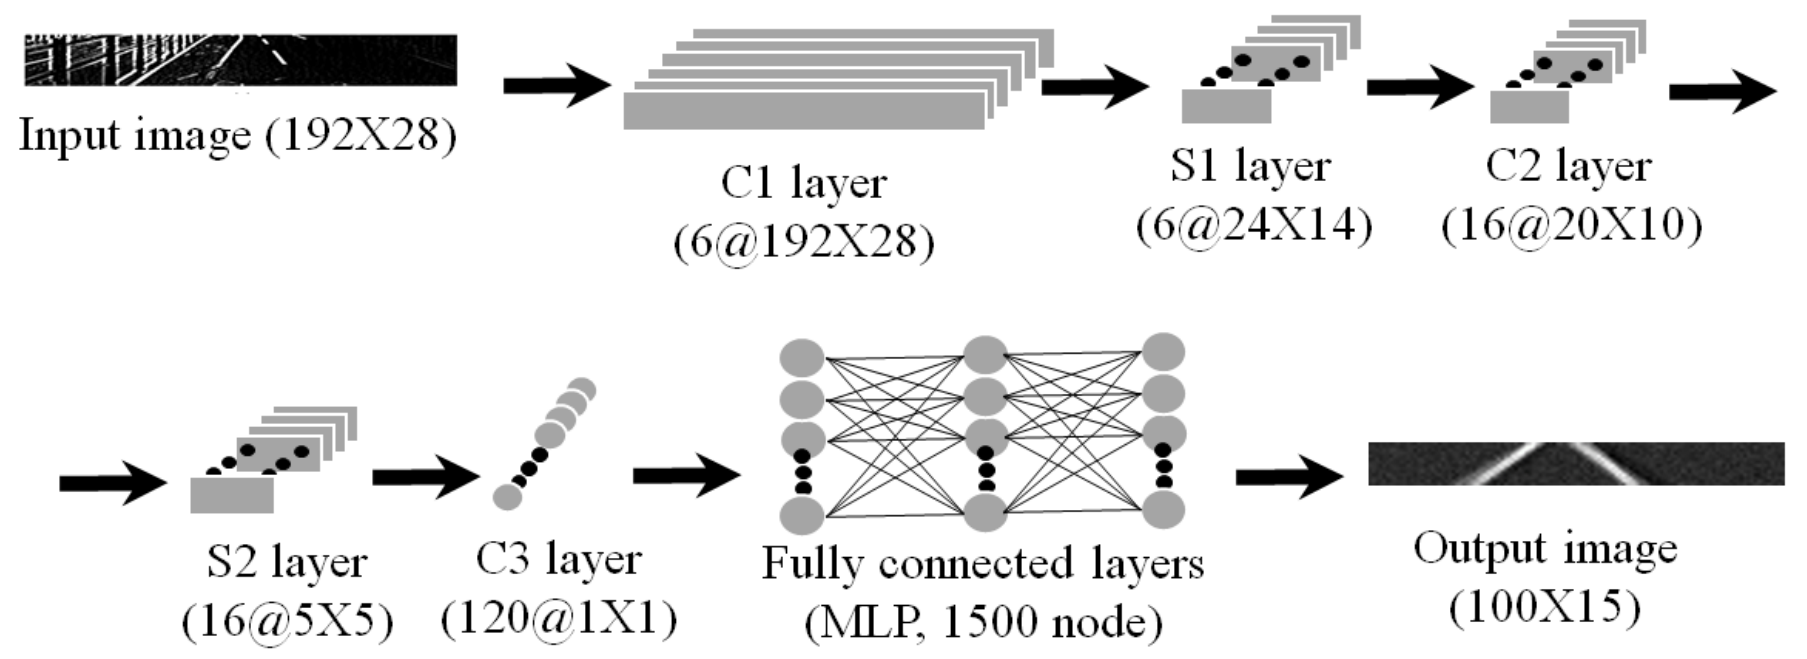
\includegraphics[width=\textwidth]{figs/cnn_map.png}
    \end{center}
    \caption{Arquitectura de CNN para predecir máscara de carril en \cite{Kim2014}.}
    \label{fig:cnn_map}
\end{figure}

\noindent\textbf{Métodos de una etapa.} Los métodos de una etapa ofrecen directamente el modelo de las líneas a partir de la imagen de entrada. Son los métodos que actualmente consiguen mejores resultados y tienen mayor velocidad. En \cite{van2019end} se propone un método que, usando una sola arquitectura neuronal, hace la detección y la regresión de los parámetros de las líneas del carril. La arquitectura consiste en dos componentes: una red neuronal profunda que predice un mapa de pesos similar a la segmentación por cada línea, y un módulo de ajuste de mínimos cuadrados diferenciable que devuelve para cada mapa los parámetros de la curva que mejor se aproxime. Por lo tanto, la red aprende a generar características que evitan inestabilidades durante la etapa de ajuste de los modelos a las líneas. 

LaneATT \cite{tabelini2021keep} propone un método basado en \textit{anchors} típico en detección de objetos (YOLO \cite{redmon2016you}, SSD \cite{liu2016ssd}), pero en vez de usar \textit{bounding boxes} usa líneas. Define un \textit{anchor} como una \textit{línea virtual} en el plano imagen compuesta por un punto de origen y una dirección. La Figura \ref{fig:late_att} muestra un esquema general del método. Se usa una CNN (ResNet \cite{he2016deep}) como \textit{backbone} para extraer características de la imagen de entrada, después cada \textit{anchor} se proyecta sobre el mapa de características, esta proyección se concatena con otro conjunto de características generado por un modelo de atención y, por último, hay dos cabezales que realizan las predicciones finales: uno de clasificación para dar la probabilidad de ser línea, y otro de regresión para ofrecer los parámetros de localización de la línea. Se utiliza el modelo de atención, que es una red densa que genera características que agregan información global, porque la información del vector de características de la proyección suele ser información local y no es suficiente para realizar predicciones en situaciones con oclusiones o líneas de carril borradas.

\begin{figure} [h]
    \begin{center}
        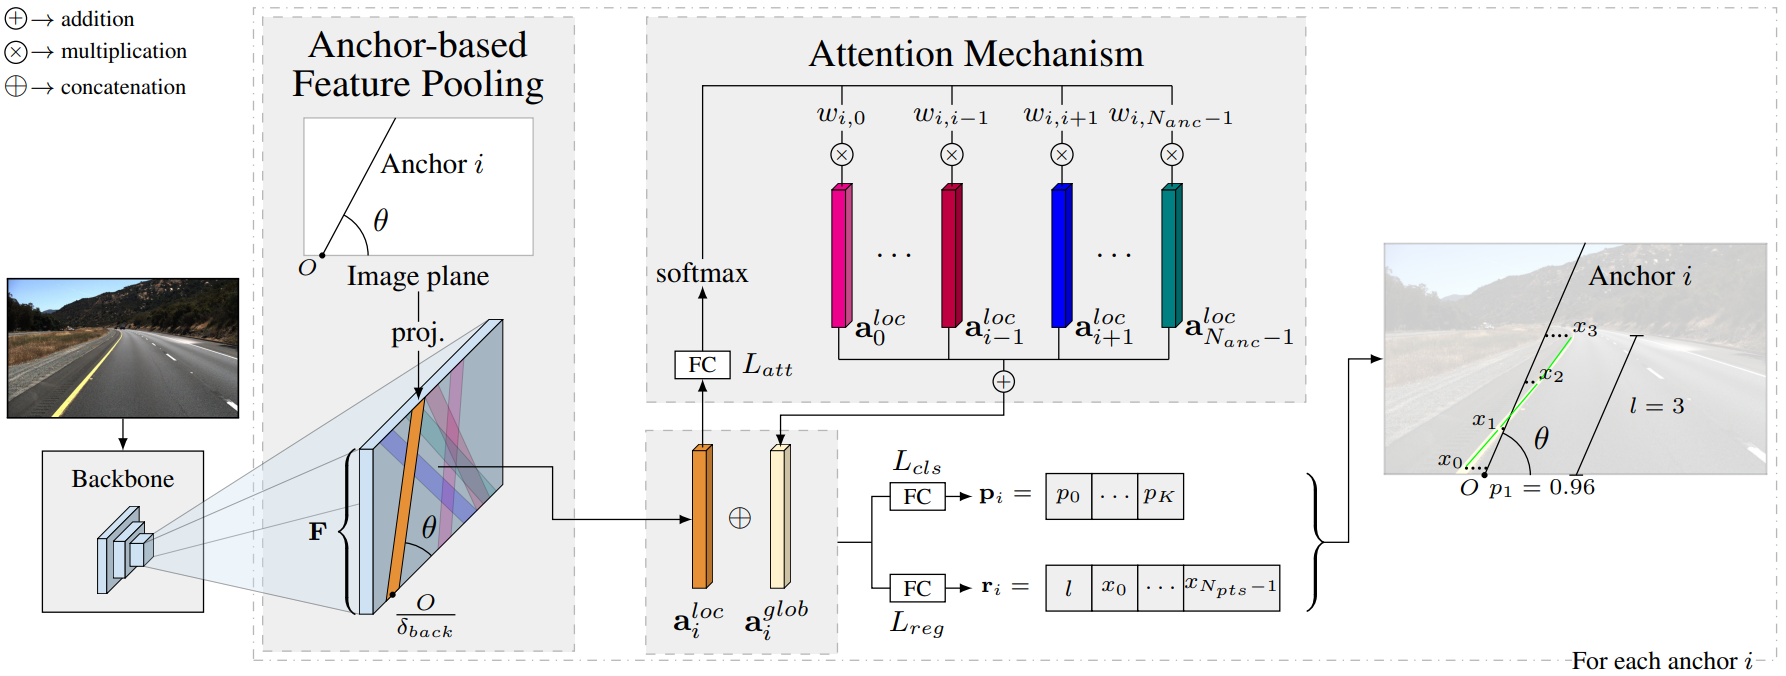
\includegraphics[width=\textwidth]{figs/laneAtt.png}
    \end{center}
    \caption{Esquema del método LaneATT \cite{tabelini2021keep}.}
    \label{fig:late_att}
\end{figure}

CLRNet \cite{zheng2022clrnet} se basa en la misma idea que LaneATT \cite{tabelini2021keep}, pero utiliza una pirámide de características para obtener la información local y global y, de esta manera, mejora la precisión de la localización. UFLD \cite{Qin2020} propone el método más rápido del estado del arte. Como se muestra en la Figura \ref{fig:lane_rows}, consiste en dividir la imagen en filas, cada fila en diferentes celdas y por cada celda ofrecer una probabilidad de contener línea o no. Cada celda se corresponde con un píxel del tensor de salida de una CNN, en este caso usan ResNet \cite{he2016deep}. De esta manera, sólo se están clasificando regiones que indican la localización de las líneas en cada fila y, por lo tanto, se está reduciendo el coste computacional. Además, en la función de pérdida se utiliza información a priori de la forma y dirección de las líneas para solucionar problemas de oclusiones. Es un método muy rápido, pero no tan preciso comparado con las demás técnicas.

\begin{figure} [h!]
    \begin{center}
      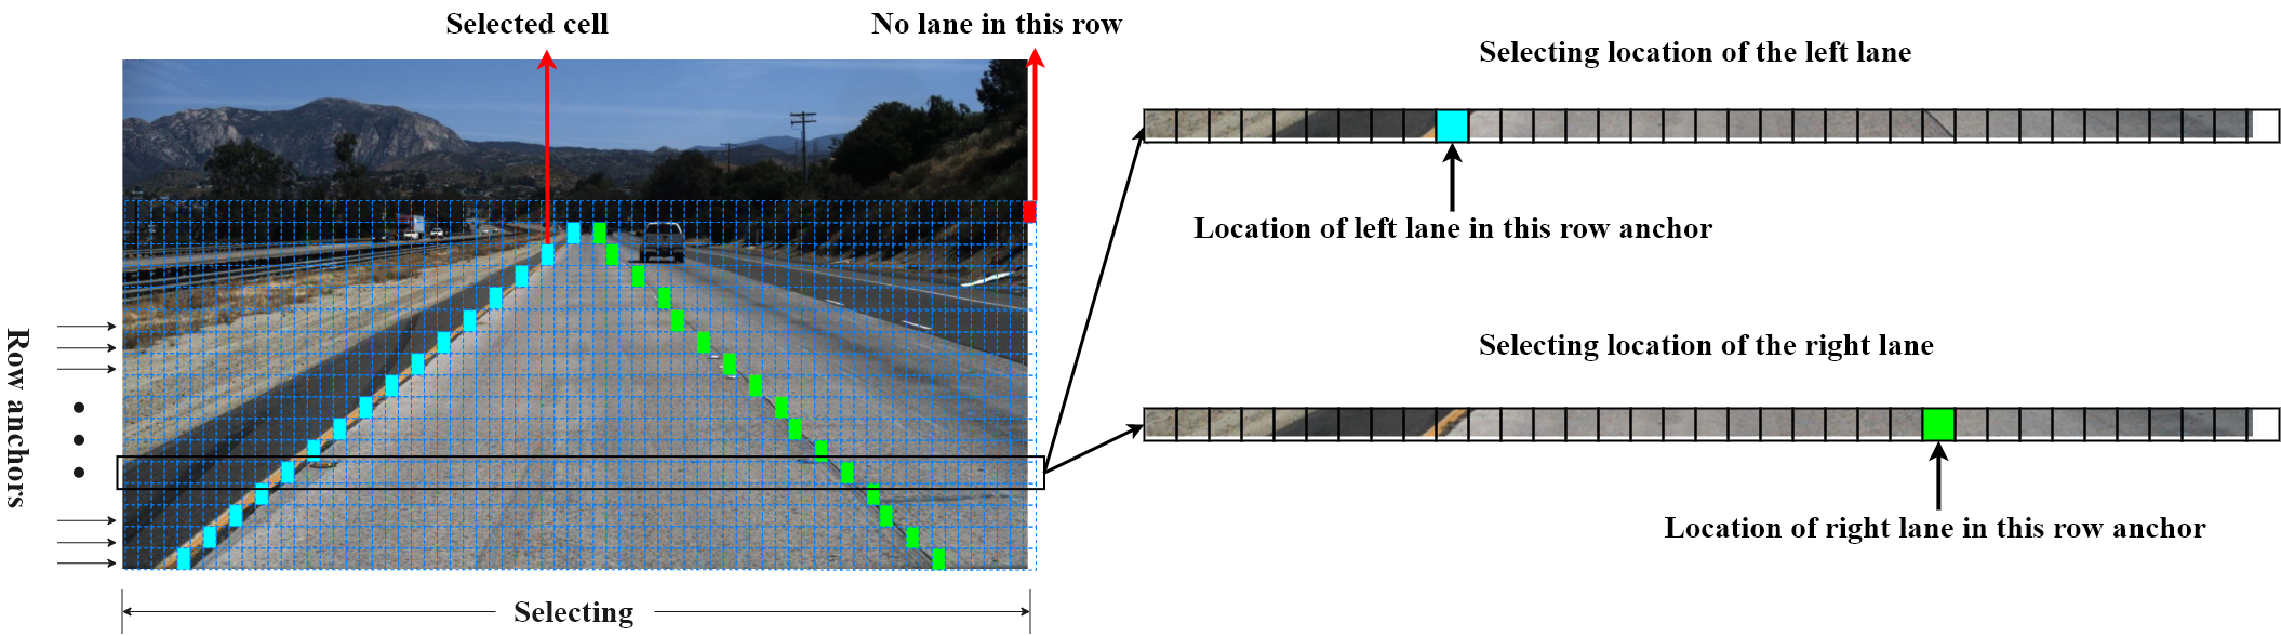
\includegraphics[width=\textwidth]{figs/lane-rows.png}
    \end{center}
    \caption{Algoritmo basado en filas de UFLD \cite{Qin2020}.}
    \label{fig:lane_rows}
\end{figure}

En la Tabla \ref{table:metodos_lane} se realiza una comparativa de precisión y rendimiento de los métodos explicados en esta sección. Para compararlos se ha usado el dataset CULane \cite{Pan2018} (Figura \ref{fig:culane}) porque contiene imágenes urbanas y el objetivo de \textit{BusVigia 2.0} es obtener la mayor precisión en esos entornos. Además, es el dataset más popular del estado del arte junto a Tusimple \cite{tusimple}, que está compuesto por imágenes capturadas en autopistas.

\begin{table}
\begin{center}
\begin{adjustbox}{width=\textwidth}
\begin{tabular}{l c c c c c c c c c c c}
\hline
Method & Backbone & FPS & Normal & Crowded & Dazzle & Shadow & No line & Arrow & Curve & Cross & Night \\
\hline
SCNN \cite{Pan2018} & VGG16 & 7.5 & 90.60 & 69.70 & 58.50 & 66.90 & 43.40 & 84.10 & 64.40 & 1990 & 66.10 \\
LaneATT \cite{tabelini2021keep} & ResNet18 & 153 & 91.17 & 72.71 & 65.82 & 68.03 & 49.13 & 87.82 & 63.75 & 1020 & 68.58 \\
LaneATT \cite{tabelini2021keep} & ResNet34 & 129 & 92.14 & 75.03 & 66.47 & 78.15 & 49.39 & 88.38 & 67.72 & 1330 & 70.72 \\
LaneATT \cite{tabelini2021keep} & ResNet122 & 20 & 91.74 & 76.16 & 69.47 & 76.31 & 50.46 & 86.29 & 64.05 & 1264 & 70.81 \\
UFLD \cite{Qin2020} & ResNet18 & \textbf{282} & 87.70 & 66.00 & 58.40 & 62.80 & 40.20 & 81.00 & 57.90 & 1743 & 62.10 \\
UFLD \cite{Qin2020} & ResNet34 & 170 & 90.70 & 70.20 & 59.50 & 69.30 & 44.40 & 85.70 & 69.50 & 2037 & 66.70 \\
CLRNet \cite{zheng2022clrnet} & ResNet18 & 119 & 93.30 & 78.33 & 73.71 & 79.66 & 53.14 & 90.25 & 71.56 & 1321 & 75.11 \\
CLRNet \cite{zheng2022clrnet} & ResNet34 & 103 & 93.49 & 78.06 & 74.57 & 79.92 & 54.01 & 90.59 & 72.77 & 1216 & 75.02 \\
CLRNet \cite{zheng2022clrnet} & ResNet101 & 46 & \textbf{93.85} & 78.78 & 72.49 & 82.33 & 54.50 & 89.79 & \textbf{75.57} & 1262 & \textbf{75.51} \\
CLRNet \cite{zheng2022clrnet} & DLA34 & 94 & 93.73 & \textbf{79.59} & \textbf{75.30} & \textbf{82.51} & \textbf{54.58} & \textbf{90.62} & 74.13 & 1155 & 75.37 \\
\hline
\end{tabular}
\end{adjustbox}
\end{center}
\caption{Evaluación de los métodos de detección de carril en el dataset CULane \cite{Pan2018} usando la métrica F1. En la categoría \textit{Cross} se muestra el número de falsos positivos. Para la comparación de FPS se ha usado una GPU NVIDIA 1080Ti.}
\label{table:metodos_lane}
\end{table}

\begin{figure} [h!]
    \begin{center}
      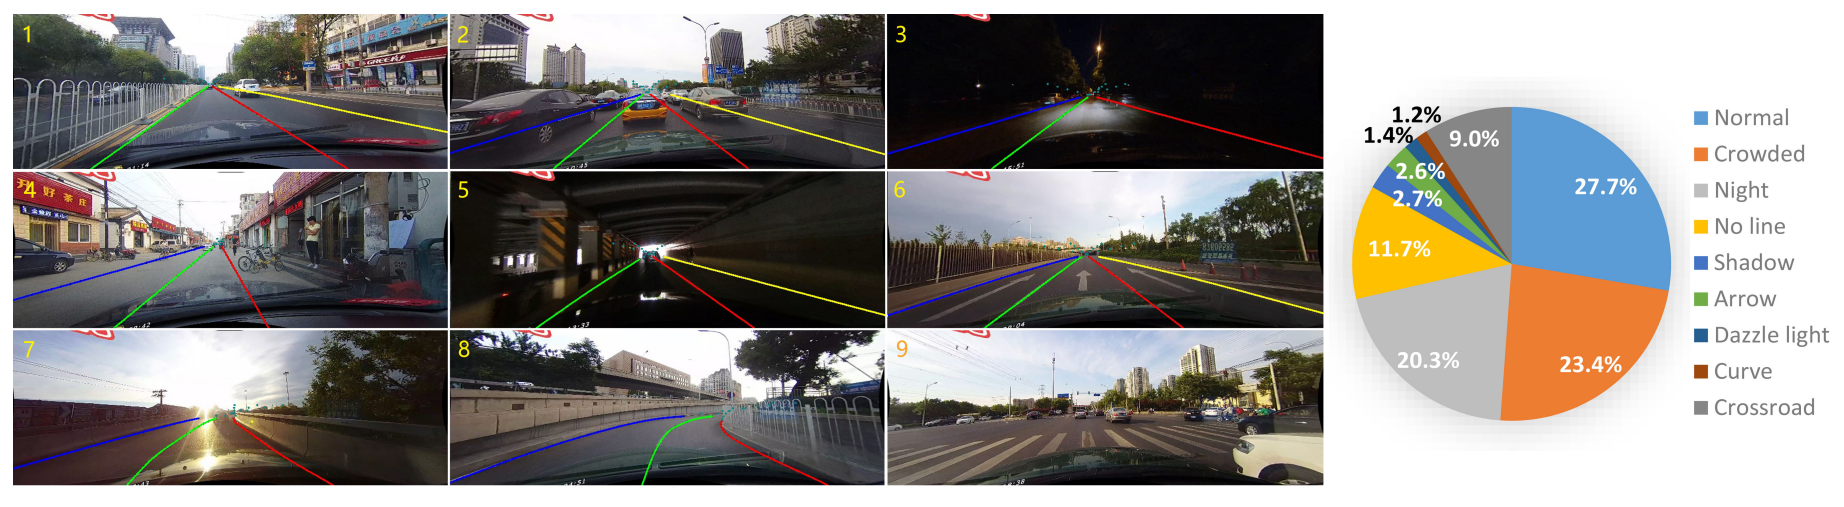
\includegraphics[width=\textwidth]{figs/culane.png}
    \end{center}
    \caption{Ejemplos del dataset CULane \cite{Pan2018}.}
    \label{fig:culane}
\end{figure}

\subsection{Reconocimiento automático de matrículas (ALPR)}

Un sistema de reconocimiento automático de matrículas o \textit{Automatic License Plate Recognition} (ALPR) en inglés, suele estar compuesto de dos etapas principales: detección de coche-matrícula y reconocimiento de matrícula.\\

\noindent\textbf{Detección de coche-matrícula.} La etapa de detección coche-matrícula tiene como objetivo obtener la regiones que contienen matrículas en la imagen, para ello se suelen utilizar métodos de detección de objetos. En la literatura se diferencian dos tipos de métodos: \textit{two-stage} y \textit{one-stage}. Los métodos \textit{two-stage} se basan en una primera fase de propuesta de regiones y, después, una segunda fase de clasificación de las regiones. El modelo más popular y con mejores resultados es Faster R-CNN \cite{ren2015faster}, que usa una CNN y un método basado en \textit{anchors} para proponer regiones. Los métodos \textit{one-stage} son más rápidos porque no tienen fase de propuesta de regiones y, actualmente, también son más precisos. SSD \cite{liu2016ssd}, FCOS \cite{tian2019fcos}, RetinaNet \cite{lin2017focal} y la familia YOLO \cite{redmon2016you} son los modelos más populares. En los trabajos \cite{laroca2018robust, laroca2021efficient} primero se detecta el vehículo usando un detector de objetos y después la matrícula usando otro, lo que incrementa el coste computacional. Se hacía de esta manera porque los modelos tenían problemas para detectar objetos pequeños. Actualmente esto ya no es un problema, modelos como YOLOv5 \cite{yolov5} detectan objetos pequeños.\\

\noindent\textbf{Reconocimiento de matrícula.} La etapa de reconocimiento de matrícula consiste en leer los caracteres alfanuméricos de las regiones obtenidas en la etapa anterior. Los métodos tradicionales \cite{Du2013} primero realizaban una segmentación de los caracteres usando, por ejemplo, umbralización \cite{miyamoto1991vehicle} o información de los bordes \cite{capar2006concurrent}, y posteriormente un reconocimiento de los caracteres usando, por ejemplo, filtros de Gabor \cite{hu2002recognition}. Los métodos modernos basados en aprendizaje profundo pueden hacer la segmentación y reconocimiento de una sola vez. En \cite{Menotti2014} usan una CNN random para extraer características de los caracteres. En \cite{Wang2019} se propone un método basado en \textit{Convolutional Recurrent Neural Network} (CRNN) y \textit{Connectionist Temporal Classification} (CTC) \cite{shi2016end} que reconoce caracteres a partir de una imagen recortada de matrícula. En \cite{montazzolli2017real} se propone CR-NET como una CNN para segmentar y reconocer, que durante varios años ha sido uno de los métodos de referencia en el estado del arte. Trabajos como \cite{laroca2018robust} o \cite{laroca2021efficient} hacen uso de CR-NET.

\begin{figure} [h]
    \begin{center}
      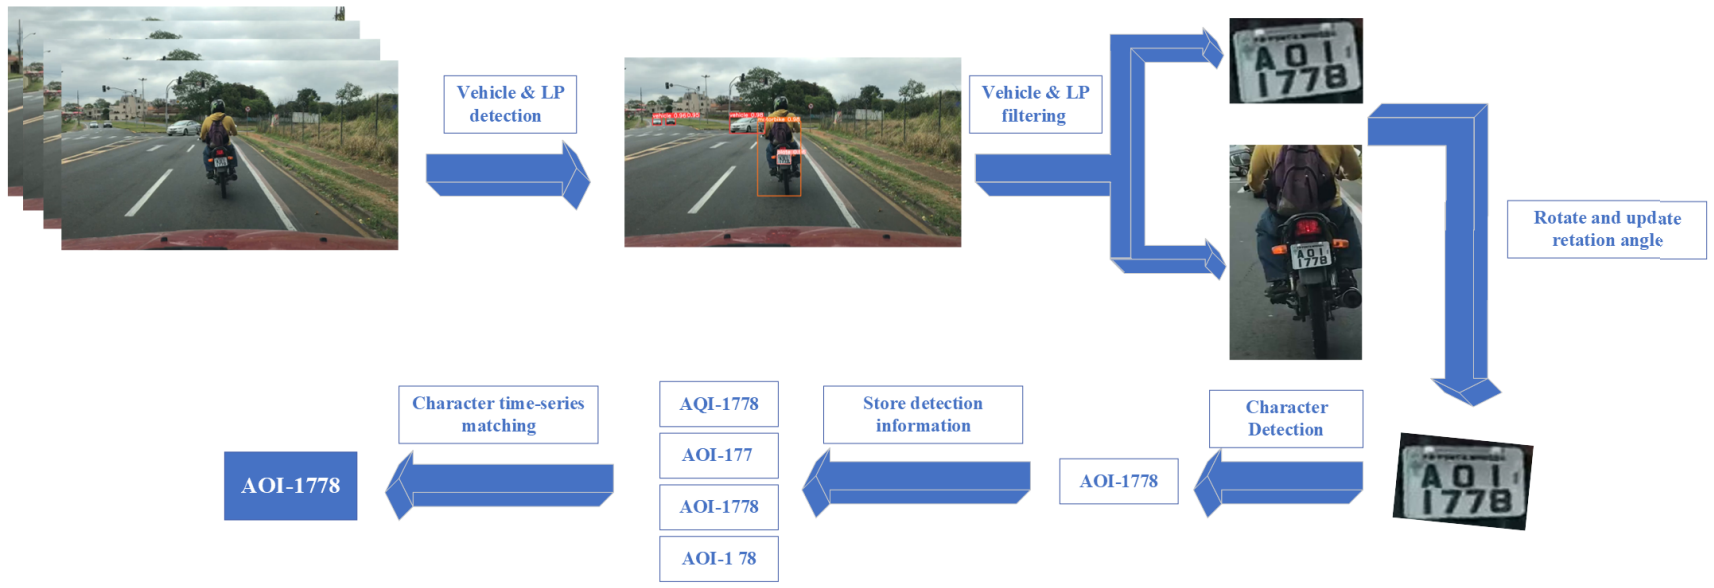
\includegraphics[width=\textwidth]{figs/alpr.png}
    \end{center}
    \caption{Sistema ALPR de \cite{Quang2022}.}
    \label{fig:alpr}
\end{figure}

En entornos reales, procesar un único \textit{frame} suele provocar resultados erróneos. En \cite{Quang2022} se hace frente a este problema usando un algoritmo que combina información de los caracteres en secuencias de \textit{frames}. Actualmente se puede considerar el método más preciso del estado del arte. La Figura \ref{fig:alpr} muestra un esquema general del sistema. Usan YOLOv5 para detectar el vehículo y la matrícula al mismo tiempo. Todas las matrículas detectadas se almacenan y ordenan por tiempo en una cola, y después se usa un algoritmo para corregir la posible rotación que hayan sufrido. Para el reconocimiento de caracteres presentan un modelo basado en YOLOv5 reduciendo el número de filtros de cada capa para ganar velocidad y eliminando el cabezal de detección para características pequeñas y medianas, ya que los caracteres son grandes dentro de la región de la matrícula. Por último, usan su algoritmo \textit{Character Time-series Matching} (CTM) que utiliza la información de una matrícula en varios \textit{frames} consecutivos para realizar una predicción final.

\begin{table}[h!]
\begin{center}
\begin{tabular}{l c}
\hline
Method & Accuracy \\
\hline
\cite{laroca2018robust} & 64.89 \\
\cite{laroca2021efficient} & 90 \\
\cite{Quang2022} & 96.7 \\
\hline
\end{tabular}
\end{center}
\caption{Evaluación de los métodos de ALPR en el dataset UFPR-ALPR \cite{laroca2018robust} usando la métrica \textit{accuracy}.}
\label{table:metodos_alpr}
\end{table}

En la Tabla \ref{table:metodos_alpr} se comparan los métodos que han sido evaluados en el dataset UFPR-ALPR \cite{laroca2018robust}. Actualmente es el dataset más complicado del estado del arte, compuesto por secuencias de vídeo en escenas realistas (Figura \ref{fig:ufpr}).

\begin{figure} [h]
    \begin{center}
      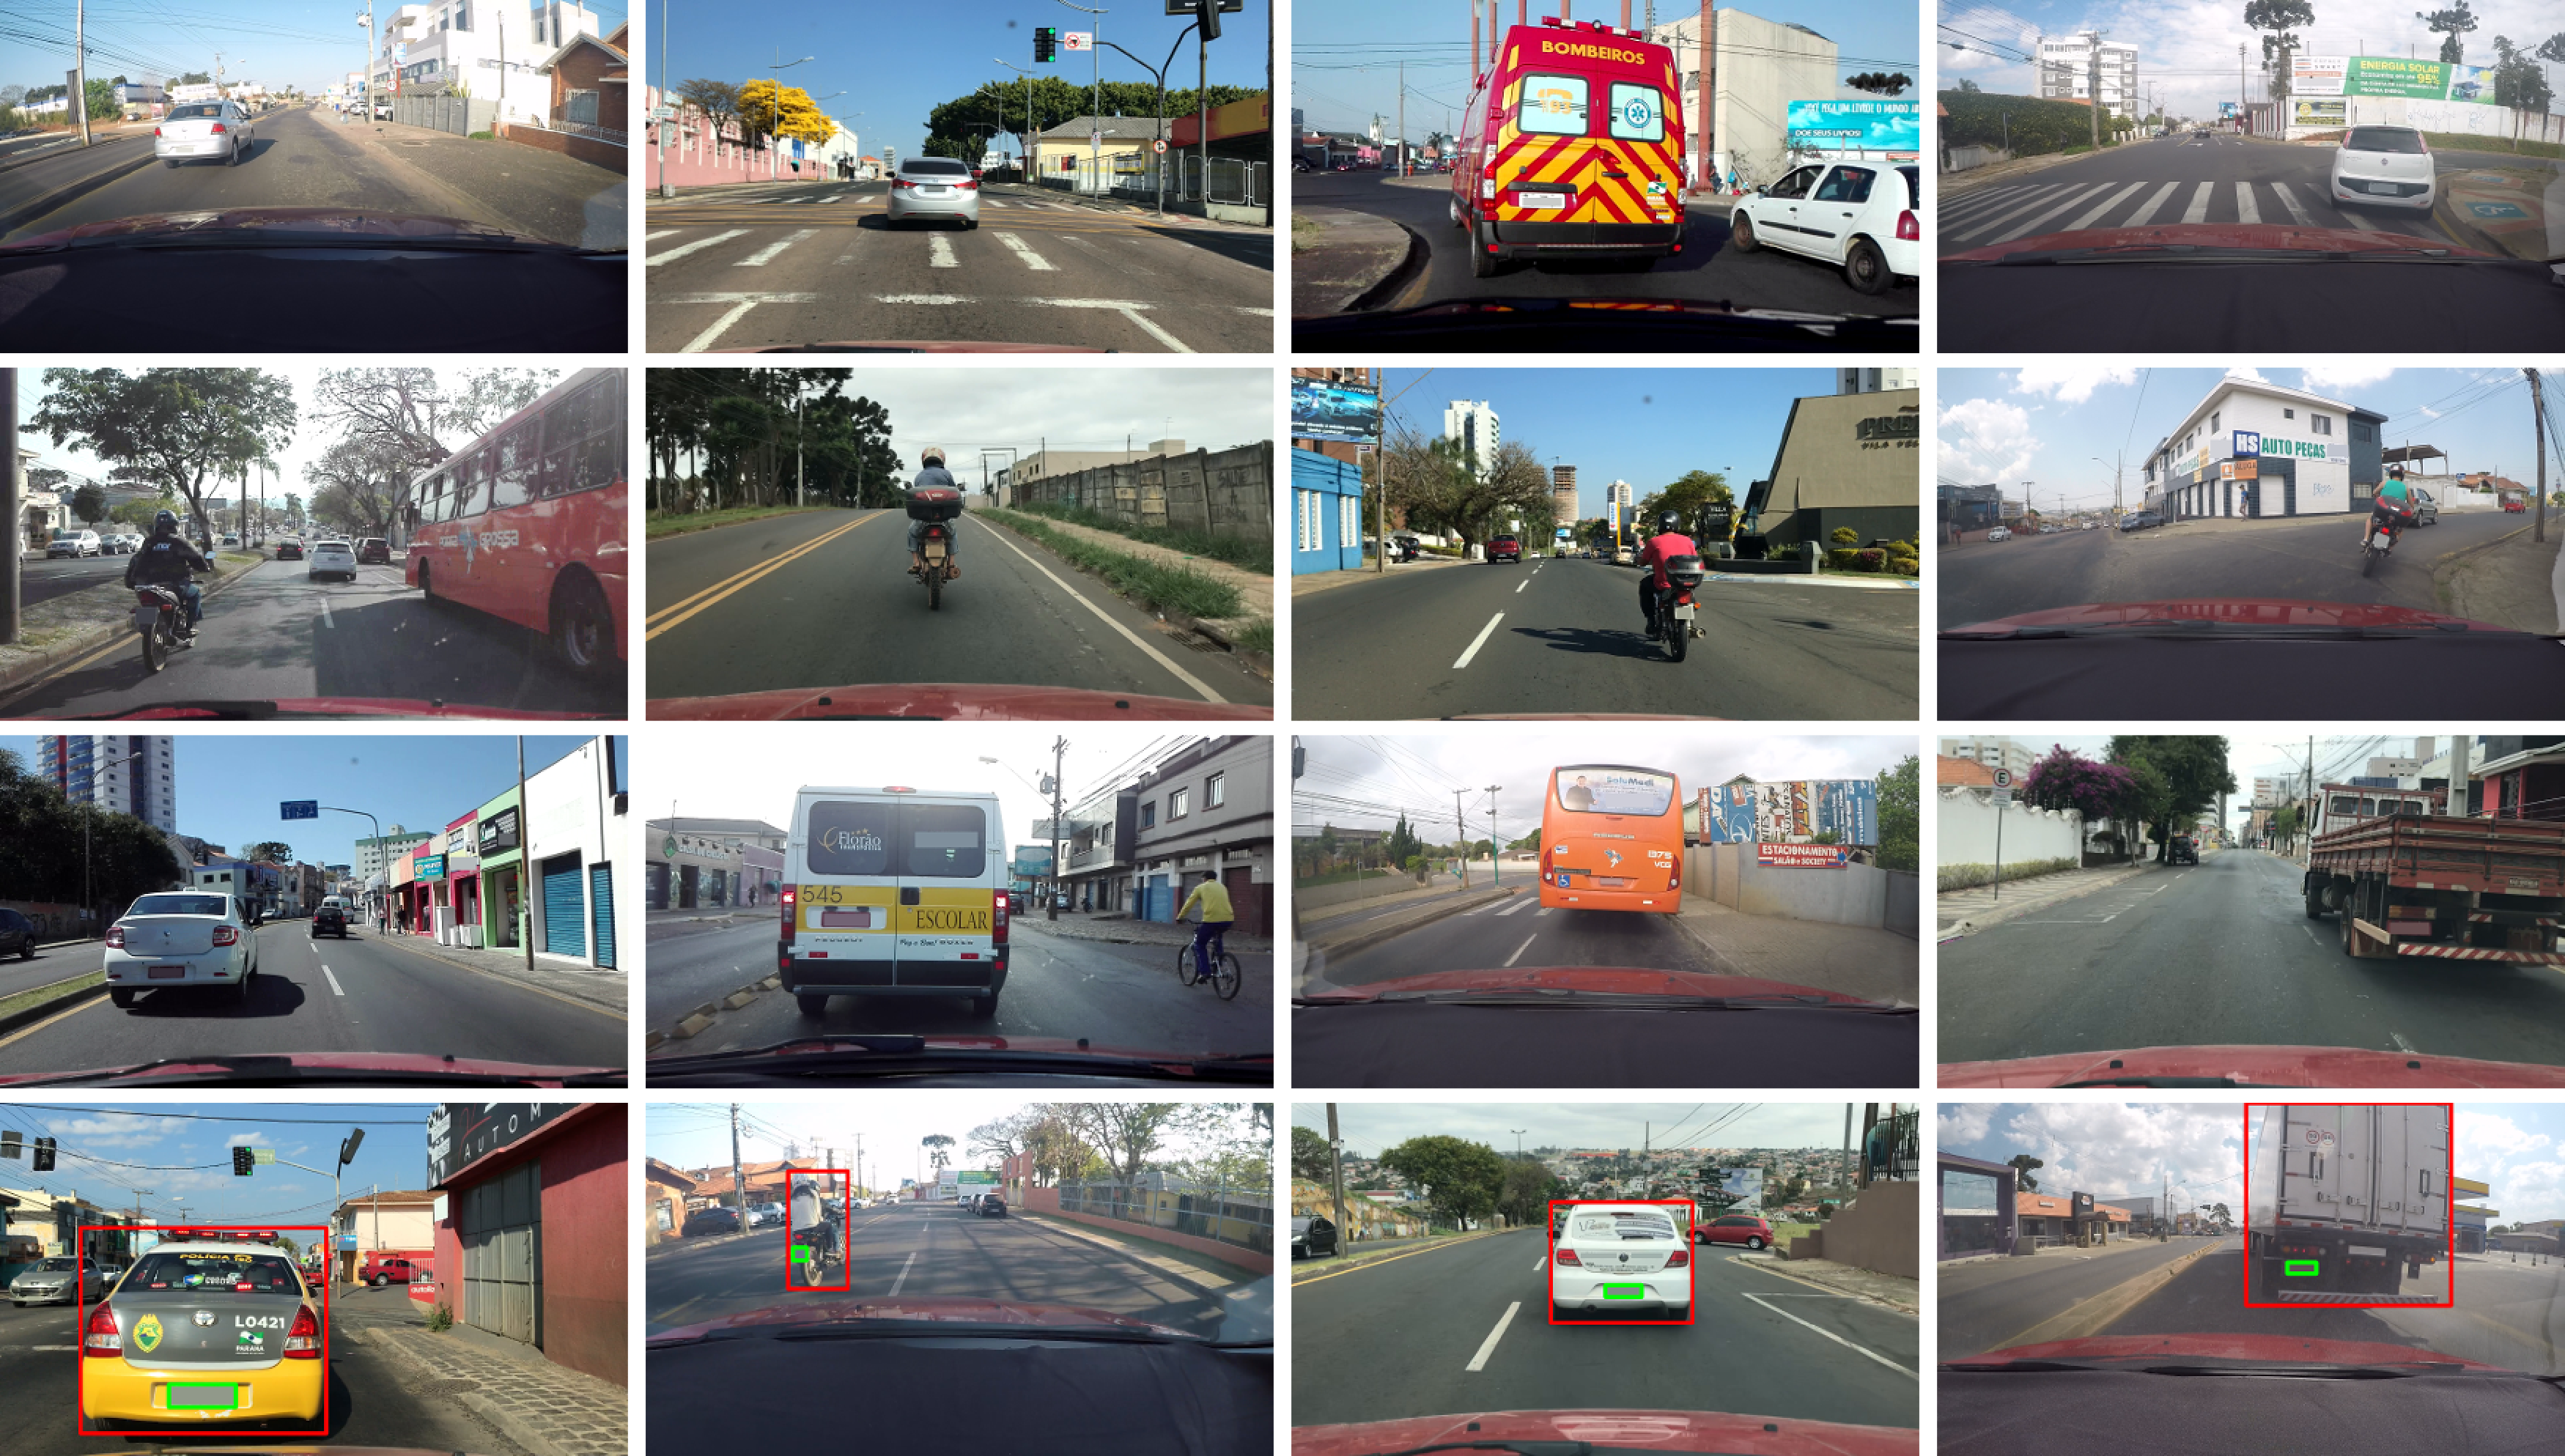
\includegraphics[width=\textwidth]{figs/ufpr.png}
    \end{center}
    \caption{Ejemplos del dataset UFPR-ALPR \cite{laroca2018robust}. La última fila son ejemplos de anotaciones.}
    \label{fig:ufpr}
\end{figure}

\clearpage
\thispagestyle{empty}
\bibliographystyle{apalike} \bibliography{bibliography}

\end{document}
